%%%%%%%%%%%%%%%%%%%%%%%%%%%%%%%%%%%%%%%%%%%%%%%%%%%%%%%%%%%%%%%%
% Thesis proposal, University of Amsterdam 
% Lukas Snoek, lukassnoek@gmail.com
%
% The title-page template was downloaded from 
% latextemplates.com and adapted to fit the
% RMP thesis proposal form. 
%
% Original author title-page template:
% WikiBooks (http://en.wikibooks.org/wiki/LaTeX/Title_Creation)
% CC BY-NC-SA 3.0 (http://creativecommons.org/licenses/by-nc-sa/3.0/)
%

%%%%%%%%%%%%%%%%%%%%%%%%%%%%%%%%%%%%%%%%%%%%%%%%%%%%%%%%%%%%%%%%
% START PRE-AMBLE
\documentclass[12pt,a4paper]{article}\usepackage[]{graphicx}\usepackage[]{color}
%% maxwidth is the original width if it is less than linewidth
%% otherwise use linewidth (to make sure the graphics do not exceed the margin)
\makeatletter
\def\maxwidth{ %
  \ifdim\Gin@nat@width>\linewidth
    \linewidth
  \else
    \Gin@nat@width
  \fi
}
\makeatother

\definecolor{fgcolor}{rgb}{0.345, 0.345, 0.345}
\newcommand{\hlnum}[1]{\textcolor[rgb]{0.686,0.059,0.569}{#1}}%
\newcommand{\hlstr}[1]{\textcolor[rgb]{0.192,0.494,0.8}{#1}}%
\newcommand{\hlcom}[1]{\textcolor[rgb]{0.678,0.584,0.686}{\textit{#1}}}%
\newcommand{\hlopt}[1]{\textcolor[rgb]{0,0,0}{#1}}%
\newcommand{\hlstd}[1]{\textcolor[rgb]{0.345,0.345,0.345}{#1}}%
\newcommand{\hlkwa}[1]{\textcolor[rgb]{0.161,0.373,0.58}{\textbf{#1}}}%
\newcommand{\hlkwb}[1]{\textcolor[rgb]{0.69,0.353,0.396}{#1}}%
\newcommand{\hlkwc}[1]{\textcolor[rgb]{0.333,0.667,0.333}{#1}}%
\newcommand{\hlkwd}[1]{\textcolor[rgb]{0.737,0.353,0.396}{\textbf{#1}}}%

\usepackage{framed}
\makeatletter
\newenvironment{kframe}{%
 \def\at@end@of@kframe{}%
 \ifinner\ifhmode%
  \def\at@end@of@kframe{\end{minipage}}%
  \begin{minipage}{\columnwidth}%
 \fi\fi%
 \def\FrameCommand##1{\hskip\@totalleftmargin \hskip-\fboxsep
 \colorbox{shadecolor}{##1}\hskip-\fboxsep
     % There is no \\@totalrightmargin, so:
     \hskip-\linewidth \hskip-\@totalleftmargin \hskip\columnwidth}%
 \MakeFramed {\advance\hsize-\width
   \@totalleftmargin\z@ \linewidth\hsize
   \@setminipage}}%
 {\par\unskip\endMakeFramed%
 \at@end@of@kframe}
\makeatother

\definecolor{shadecolor}{rgb}{.97, .97, .97}
\definecolor{messagecolor}{rgb}{0, 0, 0}
\definecolor{warningcolor}{rgb}{1, 0, 1}
\definecolor{errorcolor}{rgb}{1, 0, 0}
\newenvironment{knitrout}{}{} % an empty environment to be redefined in TeX

\usepackage{alltt}
\usepackage[utf8]{inputenc}
\usepackage{amssymb}
\usepackage{eurosym}
\usepackage[colorlinks=false,hidelinks = true]{hyperref}
\usepackage[capposition=top]{floatrow}
\usepackage{natbib}
\bibliographystyle{apalike}

\usepackage{setspace} 
\setlength{\parindent}{10mm}

\usepackage{graphicx}
\graphicspath{ {images/} }

% Header style
\usepackage{fancyhdr}
\pagestyle{fancy}
\fancyhf{}
\renewcommand{\headrulewidth}{0pt}
\lfoot{Graduate School of Psychology}
\rfoot{Page \thepage}
\IfFileExists{upquote.sty}{\usepackage{upquote}}{}
\begin{document}

%%%%%%%%%%%%%%%%%%%%%%%%%%%%%%%%%%%%%%%%%%%%%%%%%%%%%%%%%%%%%%%%
% Start titlepage environment
\begin{titlepage}

\newcommand{\HRule}{\rule{\linewidth}{0.5mm}} 
\center 

% Headings
\textsc{\LARGE Graduate School of Psychology}\\[1cm] 
\textsc{\Large University of Amsterdam}\\[1cm]

% Title section
\HRule \\[0.4cm]
{ \huge \bfseries Research Master's Psychology Thesis Proposal Form}\\[0.4cm] 
\HRule \\[1.5cm]
 
% Author section & version/data info
\begin{minipage}{0.4\textwidth}
\begin{flushleft} \large
\emph{Author:}\\
Lukas \textsc{Snoek} 
\end{flushleft}
\end{minipage}
~
\begin{minipage}{0.4\textwidth}
\begin{flushright} \large
\emph{Version:} \\
\textsc{1st draft} 
\end{flushright}
\end{minipage}\\[1cm]

% Logo

\includegraphics[width=60mm]{uva_logo_inv}\\[1cm] 

% Data
{\large \today}\\[2cm]

\vfill 

\end{titlepage}

%%%%%%%%%%%%%%%%%%%%%%%%%%%%%%%%%%%%%%%
% KNITR stuff



%%%%%%%%%%%%%%%%%%%%%%%%%%%%%%%%%%%%%%%%
% Texcount 
\newcommand\wordcount{\immediate\write18{texcount -sub=section \jobname.tex  | grep "Section" | sed -e 's/+.*//' | sed -n \thesection p > 'count.txt'}Word count: \input{count.txt}}

%%%%%%%%%%%%%%%%%%%%%%%%%%%%%%%%%%%%%%%%
% Begin actual proposal form
\onehalfspacing

\section{Who and Where?}
\vspace{\baselineskip}

\begin{tabular}{l l l}
\textbf{Student} \\
Name & : &                              Lukas Snoek\\
Student ID number & : &                 10126228 \\
Address & : &                           Commelinstraat 332 \\
Postal code and residence & : &         1093VD, Amsterdam \\
Telephone number & : &                  +31647769183 \\
Email address & : &                     lukassnoek@gmail.com \\[0.5cm]

\textbf{Supervisor(s)} \\
Within ResMas (obligatory) & : &        Dr. H.S. Scholte \\
Specialisation & : &                    Brain \& Cognition \\
%External supervisor(s), if any & : &    n/a \\
Second assessor & : &                   Prof. dr. R. Ridderinkhof \\[0.5cm]

\textbf{Misc.} \\
Research center / location & : &        Spinoza centre for neuroimaging \\
Number of credits & : &                 28 \\
%\textit{At least 25 ec} \\[0.5cm]
Ethics committee reference code & : &   2015-BC-4120 \\
%\textit{https://www.lab.uva.nl/ce/} \\[0.5cm]

\end{tabular}

%%%%%%%%%%%%%%%%%%%%%%%%%%%%%%%%%%%%%%%%
\section{Title and summary research project}

\subsection{Title}
Investigating the neural representation and development of emotional valence in the human brain.

\subsection{Summary of proposal \textmd{- max 150 words}}
In the past decade, cognitive neuroscience witnessed a paradigm shift from functional localization to distributed representations of psychological processes in the brain. Multivariate analyses have been a popular choice to investigate these distributed representations. In the psychological literature, however, the term ``distributeness'' has been used ambiguously and inconsistently, as multivariate representations may be present within a cluster of voxels, within a cortical lobe, or even across the entire brain. Furthermore, it is unclear whether multivariate information is always encoded at the voxel level, as is currently often assumed, or rather at the coarser scale of entire brain regions. This study's proposal aims to investigate the spatial distribution and multivariate dimensionality of emotional valence, which is hypothesized to be encoded within a multivariate set of brain regions. Furthermore, this proposal will exploratively examine how and where the representation of valence develops in the brain. This way, we aim to better our understanding how neuroimaging data relates to psychological processes. \\

\noindent
\wordcount (including title)

%%%%%%%%%%%%%%%%%%%%%%%%%%%%%%%%%%%%%%%%
\section{Project description \textmd{- max 1200 words}}
\subsection{Prior research}
% Describe prior research, a comprehensible literature review of the research field, converging upon the research questions. 
% a) Describe the state of affairs, including the theoretical framework, in the   current research field based on the existing body of literature.
% b) Clarify how the previous research eventuates into the research questions of the current proposal
A key question in the field of cognitive neuroscience is how the brain represents information. The past decades, the neuroimaging literature was dominated by studies employing univariate analyses to investigate which brain areas (de)activate during a particular psychological process of interest. These analyses are considered to be univariate, as they model each voxel in the brain separately and independently. Effectively, these types of studies aimed to localize psychological functions to particular brain areas. Consequently, researchers implicitly engaged in a type of ``neo-phrenology'' in which unique function-structure mappings were proposed \citep{poldrack2010}. For example, the amygdala became the ``fear area'' \citep{ledoux2003} and the anterior cingulate cortex became the ``conflict area'' \citep{vanveen2002}.  

In the light of our current understanding of the organization of the human brain, however, these function-structure mappings are unwarranted. First, for every purportedly selective function-structure mapping, several counter-examples exist \citep{poldrack2010}; second, and most importantly, significant (de)activation does not imply representation. In other words, the fact that a brain area activates in response to a certain stimulus does not mean that it represents (processing of) this stimulus.   

In the early 21st century, the cognitive neuroscience community gradually moved from this functional localization perspective to a more network-oriented perspective \citep{sporns2002,barrett2013}. Instead of asking \emph{which} regions (de)activate during a particular psychological process, they started asking \emph{how} brain areas or a network of brain areas encode and represent this particular process. Instead of treating individual voxels as independent sources of information, researchers realized that by modelling psychological concepts and processes as multivariate representations consisting of interdependent voxels, they could investigate how the brain truly represents, instead of responds to, information.

One of the first studies to show that the human brain encodes psychological concepts as distributed -- multivariate -- representations was described in the seminal paper by \cite{haxby2001}. They showed that different object categories were represented in a distributed fashion across the ventral visual cortex, regardless of mean activation level. Their approach, for which they used the term Multivariate Pattern Analysis (MVPA), gained popularity quickly as it appeared to provide a more sensitive analysis as opposed to univariate analyses \citep{norman2006,mahmoudi2012} and was consistent with and complemented the emerging network-oriented theoretical framework \citep{bressler2010}. Several new multivariate analyses were developed in the succeeding years, including the (successful) application of machine learning classifiers to distinguish neural representations (e.g. \citealp{cox2003}) and representational similarity analyses to characterize relations between neural patterns in a continuous, rather than discrete, manner \citep{kriegeskorte2008}. 

Currently, MVPA analyses are widespread in almost all domains of cognitive, affective, and social neuroscience. For example, in vision research, MVPA has been applied to correctly decode orientation preference at the voxel-level in striate cortex (\citealp{kamitani2005}, but see \citealp{opdebeeck2010} for a more nuanced interpretation). At a more coarse scale, researchers have shown that it is possible to decode episodic memory traces across the human hippocampus \citep{chadwick2010}. More recently, MVPA has surfaced in the social and affective neuroscience literature, in which it has been used to investigate representations of social and emotional processes. For example, \cite{kassam2013} has shown that different emotions have distinct neural patterns across the brain. It thus seems that MVPA is a useful analysis at different levels of representation and across a range of disciplines.     

% Research gap: what is the problem?
Despite the apparent utility of MVPA for different types of research, little is know about how to apply this analysis optimally in different research contexts. Currently, most MVPA analyses implicitly assume that representational information is encoded at the voxel-level, meaning that each voxel carries information which is independent from all other voxels in the representation. While this is likely the case for small-scale representations of, for example, low-level stimulus features such as orientation \cite{kamitani2005} or color \citep{brouwer2009}, the independence of voxels decreases when the spatial scale of representations increase. The study by \cite{brants2011} directly tested this hypothesis by testing the effect of spatial smoothing on voxel patterns within the ventral visual cortex. They showed that smoothing removes information about low-level stimulus features (spatial frequency) but leaves higher-level category information intact, suggesting different spatial scales for representations of different types of information.              

Given the study by \cite{brants2011}, there may be a positive association between the level of information and the spatial scale of information encoding. This would imply that representations of even higher-level psychological processes, such as emotion and motivation, will be represented at even larger spatial scales than object category information. Indeed, one study showed that representations of emotional processes are unaffected by spatial smoothing using a 10 mm kernel \citep{oosterwijk2015}. However, most known studies on higher-level representations such as emotion (e.g. \citealp{kassam2013,baucom2012}, motivation \cite{etzel2015}, and social perception \citep{corradi2014,chavez2015} do not -- a priori -- take into account the spatial scale at which their representations are encoded. The proposed study is aimed at investigating this spatial scale at which higher-level processes are encoded.       

\subsection{Key questions}
% Now state the key questions, the essence of the proposal. Here, the intended research should be connected to prior research. Testable hypotheses should be derived from the key question, and the relation between theory and research hypotheses should be clearly specified.

% a) Formulate a general relevant research question based on previous research.
Given that it is one of the major goals of cognitive neuroscience to investigate how the brain encodes and represents information, remarkably few studies on neural representations have directly examined their spatial scale. Apart from the well-defined encoding of low-level stimulus features at the level of individual voxels, few MVPA studies that focus on the representation of higher-level psychological concepts and processes have directly investigated at what level information is encoded. In the proposed research, we want to investigate the spatial scale of encoding of emotional valence, as emotional valence is known to robustly elicit a brain-wide network of highly clustered, spatially dependent voxels \citep{lindquist2015,chavez2015,kassam2013}. Essentially, we want to investigate whether emotional valence is encoded locally within voxels -- as is the case for low-level stimulus features --, globally within voxels -- as is currently assumed in brain-wide representations of higher-level psychological processes --, or globally within voxel clusters -- which assumes a larger spatial scale of information encoding. These terms will be referred to as ``local multivariate'', ``global multivariate'', and ``global univariate'' respectively (see figure 1 for a graphical representation of these concepts).       

\begin{figure}[h]
\floatfoot{\textbf{Figure 2}: Three basic types of representations, which vary in spatial distribution (local versus global) and spatial scale (univariate, implying uniformity between spatially dependent voxels, versus multivariate, implying spatially independent voxels). Strictly speaking, all patterns are multivariate, but spatial scale here refers to the level of representation within a set of brain regions.}
\centering
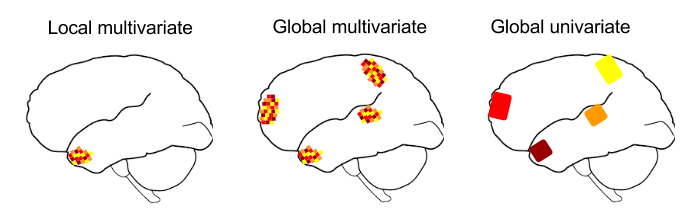
\includegraphics[scale=.55]{spatialDist}
\end{figure}

% b) Translate the general research question in a clear manner into a specific research question.
To investigate whether emotional valence is encoded as a globally univariate or multivariate representation, we will analyze its representation both as a multivariate pattern of voxels and as a multivariate pattern in which spatial dependence between voxels are taken into account by averaging activity of voxels across clusters. Put differently, we will transform the global multivariate representation into an global univariate representation. Given these two representations, we will investigate at what spatial scale -- at the level of voxels or clusters of voxels -- valence information is encoded.  Given the observed strong clustering of spatially dependent voxels in brain-wide representations of higher-level psychological processes \cite{kassam2013,oosterwijk2015,baucom2012}, we hypothesize that valence information is encoded across voxel clusters instead of individual voxels. Moreover, as averaging across spatially dependent voxels increases the pattern's signal-to-noise ratio, we predict that cluster-averaged valence representations can be better classified than the original voxel-level valence representations.  

Furthermore, as an exploratory addition to this research, we want to examine how and where the representation of valence develops in the brain over time. Questions that will be addressed, but do not bear any a priori hypotheses, include whether valence is represented as a global functional network from the beginning or gradually develop in a local-to-global fashion, and at what rate valence develops (e.g. linearly, logistically, or exponentially). Together with this study's confirmatory part on the spatial scale of valence representations, we hope to better understanding of the level of encoding of higher-level psychological processes as well as to show how, possibly, the development of these representations can be investigated over time.

\noindent
\wordcount 

%%%%%%%%%%%%%%%%%%%%%%%%%%%%%%%%%%%%%%%%
\section{Procedure \textmd{– approx. 1000 words}}
\subsection{Operationalisation}
% Describe how the research questions are operationalised. 
% a) Operationalise the research questions in a clear manner into a research design/strategy. 
To investigate the neural representation and development of valence in the brain, we want to create a novel experimental paradigm that is focused on ecological validity. To date, most studies on emotional learning and valence have used either stimuli which are inherently positively or negatively valenced (e.g. \citealp{baucom2012,aldhafeeri2012}), rendering it impossible to investigate the \emph{development} of valence, or have used neutral stimuli that are paired with unconditioned stimuli such as electric shocks \citep{visser2013}, which creates valence quickly and effectively but is not ecologically valid \citep{spiers2007}. In the experimental paradigm we aim to develop, valence will be developed in a setting that is both ecologically valid and allows for experimental control. 

In our proposed experiment, participants will be shown pictures of two exemplars of neural faces and two exemplars of visual scenes, embedded in an auditory narrative. The narrative will function to provide an ecologically valid context in which valence can be dynamically manipulated. Previous studies have demonstrated that listening to emotionally-valenced narratives robustly elicit widespread activation patterns in the brain \citep{nijhof2015,mar2011} akin to the emotion-network \citep{sabatinelli2006}. In our paradigm, the narrative will dynamically endow both the -- initially neutral -- pictures of faces and visual scenes with either positive or negative valence. We chose to manipulate two different object categories with opposing valences to create a stimulus-independent representation of valence that can be investigated with a factorial design (see section: Data analysis)

Within the narrative, the pictures of neutral faces will be consistently associated with either positive or negative valence by characterizing the faces as the narrative's ``hero'' or ``villain'' respectively. The visual scenes are similarly coupled with either a positive or negative valence by portraying one visual scene as a stereotypical ``safe house'' while the other scene is portrayed as a dangerous place. To enforce experimental control over the processing of valence, the pictures are displayed every time the characters or visual scenes are mentioned in the narrative (see figure 3). The data from this run will be used for the exploratory analyses regarding the development of valence over time.

\begin{figure}[h]
\floatfoot{\textbf{Figure 3}: The proposed experimental paradigm. The narrative is interlaced with the presentation of static images of the faces or visual scenes, whenever respectively the characters or places come up in the narrative. The images are presented 4 seconds and are not followed by an inter-trial interval.}
\centering
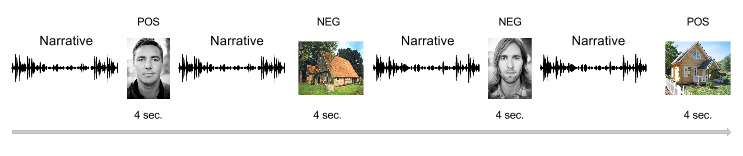
\includegraphics[scale=.55]{exp_paradigm}
\end{figure}

Moreover, we acquire a run in which subjects passively view the stimuli without a narrative, both before (pre-test) and after (post-test) the run in which valence is manipulated through the narrative. This way, we can 1) assess whether the stimuli are valence-neutral at the start of the experiment and 2) we have a robust and experimentally controlled set of responses to the by now valenced stimuli. In these runs, we use a slow event-related design in which we present each stimulus eight times for one second with an inter-stimulus interval of six seconds. The data from these runs will be used for the confirmatory part of our analyses. 

% b) Describe the procedures for conducting the research and collecting the data. 
The experimental session will last about an hour per subject. Before fMRI acquisition, subjects sign an informed consent, complete the MRI-safety screening, and are instructed about the task. As indicated previously, the fMRI scanning session will consist of three functional runs (apart from the anatomical T1 scan) as discussed previously. The first run is the ``pre-test'' run with presentation of the stimuli in a slow event-related design (approximately 4 minutes; each stimulus is presented 10 times for 1 second) without narrative. The second run will the be the run with the stimuli embedded in the narrative (approximately 20 minutes; each stimulus is presented ten times for four seconds). The last run will be the post-test, which is identical to the pre-test. During fMRI acquisition, pupil size (using an eyetracker), galvanic skin response (GSR), heart rate (power output using plethysmography), and respiration (using a respiration belt) are additionally measured as an operationalization of arousal (as a potential confounder of valence). After the scanning procedure, subjects are paid \euro 20 and debriefed about the study's research goals. 

\subsection{Sample characteristics}
% a) Indicate, given a power analysis, how many participants will be recruited. Also motivate whether the resulting number is feasible.
In this study, we will apply both univariate and multivariate (RSA and MVPA) analyses. While for univariate analyses much is known about the optimal analysis parameters, this is less so for multivariate analyses due to the their novelty. This warrants an approach in which various parameter settings -- e.g. smoothing kernel, feature selection methods, and ROI selection -- are tested for optimal use of the data \citep{kragel2012}. However, to avoid double-dipping the data, we implement the procedure originally proposed by \cite{kriegeskorte2009} in which the data is partitioned into an optimization-set and a validation-set (see figure 2). The data from the optimization-set will be used to explore various parameter settings, and when the optimal parameters are established, these will be cross-validated on the validation-set. This way, exploratory and confirmatory research can be combined to use the data optimally without double-dipping. 

This model cross-validation approach, however, comes at the cost of effectively cutting the experiment's power in half. As univariate analyses are generally less sensitive than multivariate analyses (e.g. smaller effect sizes due to stringent multiple comparison correction), the bottleneck in terms of power would be solely be determined by the univariate analysis. Fortunately, much more is known about the optimal parameters for univariate analyses. Therefore, to avoid the power bottleneck, we will perform the univariate analysis on the entire data set. This results in a sample-size of 36 for our univariate analysis, which surpasses the recommended minimum of 20 subjects for fully within-subjects, univariate fMRI analyses \citep{desmond2002}, and a sample size of 18 for our multivariate analysis. Currently, there are no guidelines concerning minimum sample size for MVPA-studies. However, our previous MVPA study on emotion-networks \citep{oosterwijk2015} yielded a satisfactory effect size (i.e. decoding accuracy 30\% above chance and a standard deviation of 11\%, Cohen's \emph{d} = 2.55) with 12 subjects (see \citealp{baucom2012}, for a similar effect size). Assuming a similar standard deviation for the results of the proposed study, a sample size of 18 subjects for the proposed study should suffice for finding a similar effect size.

\begin{figure}[t]
\floatfoot{\textbf{Figure 1}: Schematic representation of the model optimization process for the multivariate analysis. A 50/50 partitioning ratio will be used. The univariate analysis will be done \emph{once} with predetermined parameter settings and will thus not be partitioned.}
\centering
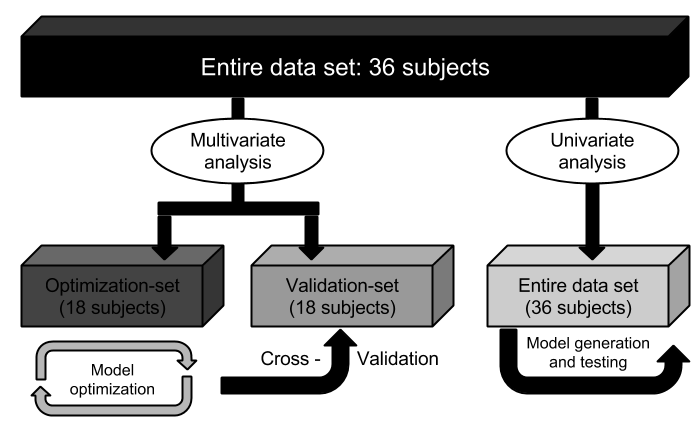
\includegraphics[scale=.5]{ModelOptimization}
\end{figure}

% b) If a subset of participants will be excluded from the analysis given their scores on dependent variables, indicate the objective criterion to do so. For example include a phrase like: “Scores on dependent variables exceeding ± 3 sd of the mean will be excluded from the analysis’’
Participants will be excluded in case of excessive movement during fMRI acquisition (\textgreater 3 millimeters within runs) and in case of falling asleep during fMRI acquisition. Participants will not be excluded based on their score on the manipulation check.

% c) If a subset of participants will be excluded from the analysis given their scores on a manipulation check item, indicate the objective criterion to do so. For example include a phrase like: “Participants scoring 15 or lower on a manipulation checks item, will be excluded from the analysis” 
% d) In case of a simulation study, indicate how data will be generated

\subsection{Materials}
% Indicate which tests, stimuli, equipment, etc. will be used; provide sufficiently elaborate descriptions and motivate your choice. (Always report the psychometric characteristics, such as reliability and validity, if existing tests are used. If new or adapted instruments or test materials (e.g., questionnaires) will be developed, then the new instrument must be independently validated first; only then it can be used as a testing instrument. Exception to this rule is allowed in case of questionnaires that do not contain more than one question (e.g., indicate on a 5-point scale how you feel today). 
Images of the two neutral faces will be drawn from the Karolinska Directed Emotional Faces (KDEF) database \citep{KDEF}, an extensively tested and validated set of pictures including images of people with valence-neutral facial expressions \citep{goeleven2008}. The visual scenes will be selected from Google images and validated in terms of valence-neutrality through an online questionnaire. In this questionnaire, subjects will indicate their association with the scenes in terms of valence (does the scene appear positive or negative?). Thirty responses on the online questionnaire will be recorded before assessing their valence-neutrality, which is operationalized as an insignificant difference in valence compared to neutral. Furthermore, stimulus-valence contingency will be fully counterbalanced between subjects (by creating four different stimulus-valence contingencies), which will eliminate any effect of initial valence.

The narrative has yet to be created. The plan is to have a professional storyteller from the Mezrab cultural center (\url{www.mezrab.nl}) create a narrative tailored to the proposed research. As discussed, the narrative should contain two characters: one who will be developed as a morally good character -- the narrative's ``hero'' -- and another who will be developed as a morally evil character -- the narrative's ``villain''. As moral goodness and evil is an inherently social concept \citep{greene2002}, this does not apply to the visual scenes. We argue that characterizing visual scenes as either ``safe'' or ``dangerous'' is equivalent to characterizing the narrative's characters as morally good or evil. The details of how to achieve this development of valence for both categories will be decided together with the storyteller. 

\subsection{Data analysis}
% Indicate for each research question separately, how it is translated into a statistical prediction. For example: “In a repeated measures ANOVA we expect an interaction effect of the between factor x and the within factor y on the dependent variable z. Also indicate how you will correct for multiple comparisons. Only the analyses proposed here can be described as confirmatory analyses in your research report. All other have to be mentioned as exploratory. 
The proposed experiment is organized as a factorial design (valence $\times$ stimulus identity) in which the representation of object categories and valence can be investigated regardless of stimulus identity. The data analysis plan and predictions will be discussed separately for the multivariate classification analysis and the multivariate RSA analysis.

\subsubsection{Confirmatory classification analysis}
In our classification analysis, we will use a support vector machine classifier to investigate whether we can distinguish between neural representations of the factors in our factorial design. For this, we will use the data from the pre- and post-test. We will use a fully data-driven dimension reduction using Fisher selection. On the resulting subset of voxels, we will employ a repeated random subsampling cross-validation approach in which we train the classifier to distinguish either between valence (positive/negative) or between stimulus category (face/visual scene). Subsequently, we average the spatially dependent voxels (using FSL's Gaussian Random Field cluster-thresholding method) and perform our classification analysis again with the reduced set of parameters (clusters instead of individual voxels). The classification analysis is done fully within subjects. The final results are based on the across-subjects averaged confusion matrix, which is statistically evaluated against chance (i.e. 50\%) using permutation statistics \citep{nichols2002}.     

\subsubsection{Exploratory RSA analysis}
The development of valence representations will be investigated using a trial-by-trial representational similarity analysis (RSA; \citealp{kriegeskorte2008}). For different feature sets (ROIs, brain-wide patterns based on Fischer selection), RSA matrices will be computed and tested using a novel model-testing method (as described in \citealp{walther2015} and demonstrated in \citealp{kornysheva2014}). As part of the exploratory analysis -- if time permits -- the covariance of pupil size and SRC, as an index of arousal, with (the development of) representations of valence is investigated.

\subsection{Modifiability of procedure}
% Is there room for modification of the intended procedure? Evaluation of the proposal by the RMP Thesis Committee is meaningful only if the recommendations that the Committee might have can be implemented. It is therefore required that the intended procedure can be modified before you start gathering data. In situations where procedures or operationalisations or sample characteristics cannot be modified, the Thesis Committee has to be consulted before handing in the research proposal. The committee will consider the eligibility of this project for a research thesis. 
The research project as proposed here can be modified along recommendations from the RMP Thesis Committee and others, in each stage of the project (preparation/stimulus materials, data acquisition, or analyses). Advice on any section of this project is very much appreciated. \\

\noindent
\wordcount

%%%%%%%%%%%%%%%%%%%%%%%%%%%%%%%%%%%%%%%%
\section{Intended results \textmd{- max 250 words}}
% Clarify what the implication of possible outcomes would be (per hypothesis) for the specific and general research questions as well as for the theory. Address the following in approximately 250 words:

% a) What are the interpretations if the results do  match the expectations? 
For our confirmatory analysis, we expect to find that classification of valence representations does not decrease when averaging over clusters of spatially dependent voxels within the entire pattern; we in fact expect that classification improves due to an increase of the representation's SNR. This finding would be interpreted as evidence for encoding of valence at the level of clusters of voxels instead of individual voxels. If averaging degrades classifier performance, then this could mean that valence information is indeed encoded at the level of voxels, regardless of their interdependence. If this coincides with at-chance classification of valence, then it is likely that our experimental paradigm failed to induce valence, in which case no conclusions about the spatial scale of the representation of valence can be drawn.  


% d) Is there any practical or societal relevance? Please explain. 
We believe that the proposed study bears a great potential to improve our fundamental understanding of functional brain networks. Ontologically, we may improve understanding of how the brain is organized functionally by showing how different psychological processes may be encoded on different spatial scales in the brain. Methodologically, we hope to show that the sensitivity of MVPA analysis may improve when a priori specifying the spatial scale on which a representation is expected. Furthermore, we hope to show that our proposed ecologically-valid experimental paradigm is a proper and effective way to investigate the development of any psychological process in the brain.  

\noindent
\wordcount

%%%%%%%%%%%%%%%%%%%%%%%%%%%%%%%%%%%%%%%%
\section{Work plan \textmd{– max 500 words}}
% Describe how the research project will be executed. Who is doing what and when? Is the planning of the current project realistic, efficient and feasible?
The research project can be conceptually divided into three stages. The preparation stage, spanning from March to mid April, will be centered around gathering the necessary stimulus materials and programming the Presentation script. This will be done in collaboration with Steven Scholte. Suzanne Oosterwijk will additionally aid in this stage because of her expertise in emotion research. In this stage I will also start programming a fully open-source preprocessing and analysis pipeline in Python, with a focus on ``literate programming'' \citep{knuth1984}, transparency, and reproducibility (as argued here: \url{http://tinyurl.com/pmveewc}). Tomas Knapen (VU University), who is very experienced Python programmer, will assist in creating the pipeline. Early April I will begin recruiting participants. 

The data acquisition stage will start mid April, when the 3T scanner at the Spinoza Centre for Neuroimaging will be fully operational again after the hardware upgrade. I plan to scan 36 participants in three weeks time. As the experimental protocol takes about 40 minutes, this will result in 8 hours per week. If there is more time available at the scanner, I will try to scan more people per week. During this stage, I will start programming the multivariate encoding analysis. Steven Scholte and Renée Visser (who is experienced with RSA analyses) will help with programming the analysis.

In the first or second week of May (depending when data acquisition is finished), the data analysis stage will start. This stage will be centered around finishing the analysis scripts and subsequently trying out different parameters on the optimization-set. In the first week of June, I hope to execute the final analysis on the validation-set and start writing my thesis report. I plan to finish a draft of my report mid July and, after revision, submit a final version at the end of the month.

\subsection{Time schedule}
% State the total amount of ec as noted in the thesis contract (25-31 ec excl. proposal), 1 ec stands for 28 hours work. Present and justify a time schedule in weeks, including your time investment in hours per week. Plan some spare time, and indicate what elements can be cut / reduced if necessary.
The project will amount to a total of 28 EC, or  784 hours. Assuming a standard 40 hours (5 day) working week, the research project will be finished the 24th of July. This allows for one week of planned vacation. In case of unplanned delay in either stage of the research project, the parameter optimization process can be shortened. 

\subsection{Infrastructure}
% Where will the research take place? How is access to the facilities and materials ensured?
Data acquisition will take place at the Spinoza Centre for Neuroimaging. As a research assistant, I have access to the centre and its facilities at all times. The centre provides all necessary equipment, including proprietary software (e.g. Presentation). 

\subsection{Budget}
% The compensation from the department is max € 80 for each research project. If the total expenditure exceeds the maximum compensation, then specify how the surplus will be financed. The € 80 budget may be used for printing costs (e.g. for the conference poster), travel expenses, participant payment. Specify the financial ramifications for the intended research. Please go to the secretariat of the specialization of your supervisor with your receipts. The secretariat will reimburse the costs you made up to € 80. 
The research project will be financed by funds of Steven Scholte. I will use approximately 30 euros of the Brain \& Cognition departmental budget to print a poster which I will present at the annual Research Master's Graduate Conference. \\

\noindent
\wordcount

%%%%%%%%%%%%%%%%%%%%%%%%%%%%%%%%%%%%%%%%
% Bibliography, natbib with apalike style 
\renewcommand{\bibsection}{} % Turn off header creation
\section{References}
\bibliography{refs}
% List all cited literature, formatted according to the directions of the APA Manual.

%%%%%%%%%%%%%%%%%%%%%%%%%%%%%%%%%%%%%%%%
\section{Further steps}
Make sure your supervisor submits an Ethics Checklist for your intended research to the Ethics Committee of the Department of Psychology at http://ce.psy-uva.nl/. Submit the research proposal in PDF by email to researchmaster-psychology@uva.nl. 
If you have the proposal signed by the supervisor(s) and you have scanned their signatures in the PDF, you only have to hand in a digital version of the proposal. However if the signatures are not on the PDF, please also submit a printed copy of the signed research proposal to the secretariat of the Research Master Psychology:
\vspace{\baselineskip}

\noindent
Universiteit van Amsterdam \\
Research Master’s Psychology \\
Weesperstraat 4, room 1.02 \\
1018 XA Amsterdam \\
researchmaster-psychology@uva.nl
\vspace{\baselineskip}

\noindent
A response of the Research Master's Thesis Committee can be anticipated within 10 workdays (i.e. two weeks) after handing in the proposal. 

%%%%%%%%%%%%%%%%%%%%%%%%%%%%%%%%%%%%%%%%
\section{Signatures}
$\square$ I hereby declare that both this proposal, and its resulting thesis, will only contain original material and is free of plagiarism (cf. Chapter 11 or the Research Master's course catalogue).
\vspace{\baselineskip}

\noindent
$\square$ I hereby declare that the result section of the thesis will consist of two subsections, one entitled ``confirmatory analyses'' and one entitled ``exploratory analyses'' (one of the two subsections may be empty):

\begin{enumerate}
\item The confirmatory analysis section reports exactly the analyses proposed in section 4 of this proposal
\item The exploratory analysis section contains additional, and thus exploratory, analyses. 
\end{enumerate}

\noindent
\textbf{Signature student:} 
\vspace*{2\baselineskip} \\
\line(1,0){175} \\

\noindent
\textbf{Signature ResMas supervisor:}
\vspace*{2\baselineskip} \\
\line(1,0){175} \\

% Uncomment if you have an external supervisor
%
% \noindent
%\textbf{Signature external supervisor (if applicable):}
%\vspace*{2\baselineskip} \\
%\line(1,0){175} \\

\end{document}
